\documentclass[a4paper, 11pt]{article}

% Packages
\usepackage[utf8]{inputenc}
\usepackage[T1]{fontenc}
\usepackage[english]{babel}
\usepackage{amsmath, amssymb, amsthm}
\usepackage{geometry}
\usepackage{graphicx}
\usepackage{hyperref}
\usepackage{algorithm}
\usepackage{algpseudocode}
\usepackage{booktabs}
\usepackage{microtype}
\usepackage{tikz}
\usetikzlibrary{matrix,positioning,arrows.meta,calc}

% Layout
\geometry{left=2.5cm, right=2.5cm, top=3cm, bottom=3cm}

% Theorems
\newtheorem{theorem}{Theorem}
\newtheorem{definition}{Definition}
\newtheorem{lemma}{Lemma}
\newtheorem{corollary}{Corollary}

% Metadata
\title{\textbf{Double Gate Extension (DGE): Decoupling Inference and Training for Perfect Continual Learning}}
\author{Dipl.-Inf. Sven Jansen}
\date{December 2024}

\begin{document}

\maketitle

\begin{abstract}
Continual learning in neural networks faces the fundamental \textbf{Plasticity-Stability Dilemma}: new learning must modify weights (plasticity), but old knowledge is encoded in those same weights (stability). We present the \textbf{Double Gate Extension (DGE)}, a novel architectural solution that \emph{decouples} these constraints through a dual-gate mechanism. Each weight matrix is controlled by two independent gate sets: \textbf{Forward Gates} ($G_{fwd}$) that control signal visibility during inference, and \textbf{Backward Gates} ($G_{bwd}$) that control gradient flow during training. This separation enables the network to \emph{use} old knowledge ($G_{fwd}$ open) while \emph{protecting} it from modification ($G_{bwd}$ closed). We prove that this provides a \textbf{mathematical guarantee} against catastrophic forgetting, not merely a regularization technique. Furthermore, we introduce a \textbf{configurable frozen core topology} that enables experimentation with different expansion patterns. DGE extends the Gated Ghost Expansion (GGE) framework while maintaining compatibility with RoPE-based architectures.
\end{abstract}

\section{Introduction: The Plasticity-Stability Dilemma}

The central challenge of continual learning can be formalized as a conflict between two objectives:

\begin{definition}[Plasticity]
The ability of a neural network to adapt its weights $W$ in response to new training data $\mathcal{D}_{new}$.
\end{definition}

\begin{definition}[Stability]
The requirement that performance on previously learned tasks $\mathcal{D}_{old}$ remains unchanged.
\end{definition}

Traditional approaches address this dilemma through:
\begin{itemize}
    \item \textbf{Regularization methods} (EWC, SI): Penalize changes to ``important'' weights
    \item \textbf{Replay methods}: Mix old data with new during training
    \item \textbf{Architecture methods}: Allocate separate capacity for each task
\end{itemize}

All these methods provide \emph{probabilistic} protection at best. We propose an \textbf{architectural guarantee}: making it physically impossible for gradients to modify protected weights.

\section{The Dual-Gate Architecture}

\subsection{Core Principle: Separate Control Channels}

For a weight matrix $W \in \mathbb{R}^{n \times k}$, we introduce two independent gate systems:

\begin{equation}
    \text{Forward Gate: } G_{fwd} = \sigma(g^{row}_{fwd} \oplus g^{col}_{fwd})
\end{equation}

\begin{equation}
    \text{Backward Gate: } G_{bwd} \in \{0, 1\}^{n \times k}
\end{equation}

Where $\oplus$ denotes the outer sum ($g^{row}_i + g^{col}_j$) and $\sigma$ is the sigmoid function.

\subsection{Forward Pass}

During inference, the effective weight matrix is:
\begin{equation}
    W_{eff} = W \odot G_{fwd}
\end{equation}

The output is computed as:
\begin{equation}
    y = W_{eff} \cdot x = (W \odot G_{fwd}) \cdot x
\end{equation}

\subsection{Backward Pass (Gradient Isolation)}

During training, we intercept the gradient update:
\begin{equation}
    \nabla W := \nabla W \odot G_{bwd}
\end{equation}

\begin{theorem}[Perfect Protection]
If $G_{bwd}[i,j] = 0$ for some weight $W[i,j]$, then $W[i,j]$ remains unchanged regardless of training dynamics.
\end{theorem}

\begin{proof}
The weight update rule is $W_{t+1} = W_t - \eta \nabla W_t$. After applying the gradient mask:
\begin{equation}
    W_{t+1}[i,j] = W_t[i,j] - \eta \cdot (\nabla W_t[i,j] \cdot G_{bwd}[i,j]) = W_t[i,j] - \eta \cdot 0 = W_t[i,j]
\end{equation}
\end{proof}

\subsection{The Key Innovation: Decoupling}

The fundamental innovation is that $G_{fwd}$ and $G_{bwd}$ are \textbf{independent}:

\begin{center}
\begin{tabular}{|c|c|l|}
\hline
$G_{fwd}$ & $G_{bwd}$ & Behavior \\
\hline
Open (1) & Open (1) & Normal: Weight is used and trainable \\
Open (1) & Closed (0) & \textbf{Protected}: Weight is used but frozen \\
Closed (0) & Open (1) & Silent: Weight contributes nothing (yet trainable) \\
Closed (0) & Closed (0) & Dormant: Weight is invisible and frozen \\
\hline
\end{tabular}
\end{center}

The ``Protected'' state is the key enabler of continual learning: old knowledge remains accessible ($G_{fwd} = 1$) but immutable ($G_{bwd} = 0$).

\section{Matrix Expansion Topology}

\subsection{Quadrant Structure}

When expanding a matrix from $\mathbb{R}^{n \times k}$ to $\mathbb{R}^{(n+\Delta n) \times (k+\Delta k)}$, we obtain four functional quadrants:

\begin{figure}[h]
\centering
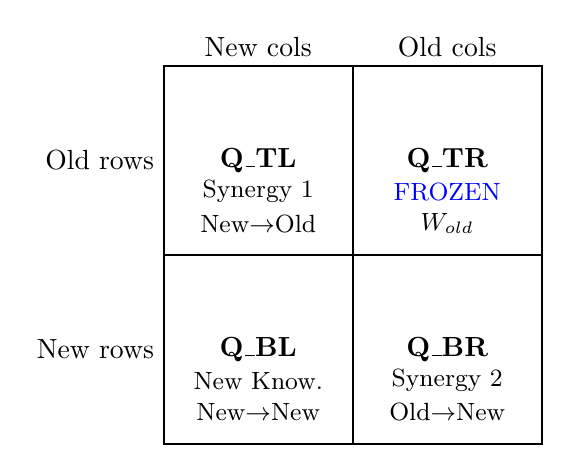
\begin{tikzpicture}[scale=0.8]
    % Draw the matrix
    \draw[thick] (0,0) rectangle (6,6);
    \draw[thick] (3,0) -- (3,6);
    \draw[thick] (0,3) -- (6,3);
    
    % Labels
    \node at (1.5,4.5) {\textbf{Q\_TL}};
    \node at (1.5,4.0) {\small Synergy 1};
    \node at (1.5,3.5) {\small New$\to$Old};
    
    \node at (4.5,4.5) {\textbf{Q\_TR}};
    \node at (4.5,4.0) {\small \textcolor{blue}{FROZEN}};
    \node at (4.5,3.5) {\small $W_{old}$};
    
    \node at (1.5,1.5) {\textbf{Q\_BL}};
    \node at (1.5,1.0) {\small New Know.};
    \node at (1.5,0.5) {\small New$\to$New};
    
    \node at (4.5,1.5) {\textbf{Q\_BR}};
    \node at (4.5,1.0) {\small Synergy 2};
    \node at (4.5,0.5) {\small Old$\to$New};
    
    % Dimension labels
    \node[above] at (1.5,6) {New cols};
    \node[above] at (4.5,6) {Old cols};
    \node[left] at (0,4.5) {Old rows};
    \node[left] at (0,1.5) {New rows};
\end{tikzpicture}
\caption{Quadrant topology of an expanded DGE weight matrix.}
\end{figure}

\subsection{Synergy Subspaces}

The non-frozen quadrants serve distinct purposes:

\begin{itemize}
    \item \textbf{Q\_TL (New Input $\to$ Old Output)}: Learns to map new data distributions into the pre-existing semantic space. Enables old capabilities to process new input modalities.
    
    \item \textbf{Q\_BL (New $\to$ New)}: Pure expansion capacity for entirely new knowledge.
    
    \item \textbf{Q\_BR (Old Input $\to$ New Output)}: Learns to repurpose old features for new objectives. Enables knowledge transfer from old to new.
\end{itemize}

\subsection{Configurable Frozen Core Position}

A key innovation of DGE is that the frozen core can be placed at \textbf{any} position in the expanded matrix:

\begin{definition}[Frozen Core Position]
$\mathcal{P} \in \{\text{TOP\_LEFT}, \text{TOP\_RIGHT}, \text{BOTTOM\_LEFT}, \text{BOTTOM\_RIGHT}, \text{CUSTOM}\}$
\end{definition}

This flexibility enables experimental investigation of different expansion topologies and their effects on knowledge transfer and synergy learning.

\section{RoPE-Invariant Head Expansion}

\subsection{The RoPE Problem}

Rotary Positional Embeddings (RoPE) encode positions through dimension-pair rotations:
\begin{equation}
    f(x_m, m) = R^d_{\Theta, m} x_m
\end{equation}

Naively expanding $d_{model}$ changes the frequency formula $\theta_i = b^{-2(i-1)/d}$ for \emph{all} dimensions, destroying learned positional understanding.

\subsection{Solution: Head Addition}

DGE expands width by adding \textbf{complete attention heads} rather than individual dimensions:
\begin{equation}
    d_{model,new} = d_{model,old} + h_{new} \cdot d_{head}
\end{equation}

Where $d_{head}$ remains constant. This preserves RoPE frequencies for all existing heads.

\begin{theorem}[RoPE Invariance]
Head addition expansion preserves the RoPE frequency basis for all legacy heads.
\end{theorem}

\begin{proof}
For legacy head $i$ with dimensions $[i \cdot d_{head}, (i+1) \cdot d_{head})$, the frequencies $\theta_j = b^{-2(j-1)/d_{head}}$ depend only on $d_{head}$, which remains unchanged.
\end{proof}

\section{Forward Gate Ramp-Up Schedule}

To prevent activation shock when introducing new capacity, forward gates follow a sigmoid schedule:

\begin{equation}
    G_{fwd}(t) = \sigma\left(20 \cdot \left(\frac{t}{T_{ramp}} - 0.5\right)\right)
\end{equation}

This provides smooth integration:
\begin{itemize}
    \item $t = 0$: $G_{fwd} \approx 0$ (new weights invisible)
    \item $t = T_{ramp}/2$: $G_{fwd} = 0.5$ (gradual activation)
    \item $t = T_{ramp}$: $G_{fwd} \approx 1$ (fully integrated)
\end{itemize}

\section{Experimental Validation}

\subsection{The "Seed Fund" Protocol}

To demonstrate DGE's capability to retain structural logic while adapting to new, semantically distinct domains, we designed a multi-stage experiment chain:

\begin{enumerate}
    \item \textbf{Phase 1 (The Child Brain):} A DGE model ($d=768$, 12 layers) is trained on \emph{TinyStories} to acquire basic causal logic and grammar.
    \item \textbf{Phase 2 (The Adaptation):} The model is expanded ($d=1024$) and trained on \emph{BBC News}. This introduces high-entropy real-world facts into the low-entropy "Child" logic.
    \item \textbf{Phase 3 (The Polyglot):} The model is further expanded ($d=1280$) and trained on \emph{German News}.
\end{enumerate}

\subsubsection{Hypothesis}
We hypothesize that a DGE-equipped model will exhibit:
\begin{itemize}
    \item \textbf{Zero Forgetting:} The "Child" logic remains accessible for simple prompting ($G_{fwd} \approx 0$ for new quadrants).
    \item \textbf{Symbiotic Transfer:} The "News" capacity utilizes the "Child" grammar ($Q_{TL}$ synergy) without overwriting it.
    \item \textbf{Language Separation:} German vocabulary does not leak into English generations unless explicitly requested (controlled by $G_{fwd}$ context).
\end{itemize}

\section{Implementation}

The DGE layer is implemented as a drop-in replacement for standard linear layers:

\begin{algorithm}
\caption{DoubleGateLinear Forward Pass}
\begin{algorithmic}[1]
\Require Input $x$, weights $W$, forward gates $g^{row}_{fwd}, g^{col}_{fwd}$
\State $G_{fwd} \gets \sigma(g^{row}_{fwd} \oplus g^{col}_{fwd})$ \Comment{Outer sum + sigmoid}
\State $W_{eff} \gets W \odot G_{fwd}$ \Comment{Element-wise masking}
\State \Return $W_{eff} \cdot x$
\end{algorithmic}
\end{algorithm}

\begin{algorithm}
\caption{Gradient Masking (Backward Hook)}
\begin{algorithmic}[1]
\Require Gradient $\nabla W$, backward mask $G_{bwd}$
\State \Return $\nabla W \odot G_{bwd}$ \Comment{Zero gradients where $G_{bwd} = 0$}
\end{algorithmic}
\end{algorithm}

\section{Theoretical Analysis}

\subsection{Comparison with GGE}

\begin{center}
\begin{tabular}{|l|c|c|}
\hline
\textbf{Property} & \textbf{GGE} & \textbf{DGE} \\
\hline
Gate count per dimension & 1 & 2 \\
Inference control & Yes & Yes \\
Training control & Coupled & \textbf{Decoupled} \\
Perfect protection & No & \textbf{Yes} \\
Flexible topology & No & \textbf{Yes} \\
\hline
\end{tabular}
\end{center}

\subsection{Complexity Analysis}

The additional memory overhead is:
\begin{equation}
    \Delta M = n + k + n \cdot k \approx n \cdot k \text{ (for the backward mask)}
\end{equation}

This is $O(1)$ relative to the weight matrix itself and can be optimized to store only region boundaries for rectangular frozen regions.

\section{Conclusion}

The Double Gate Extension provides an \textbf{architectural guarantee} against catastrophic forgetting by decoupling signal flow from gradient flow. Unlike regularization-based approaches, DGE makes it \emph{physically impossible} for training to modify protected weights. Combined with flexible frozen core placement and RoPE-invariant head expansion, DGE enables true continual learning in modern transformer architectures.

\bibliographystyle{plain}
\begin{thebibliography}{9}
\bibitem{gge} Jansen, S. (2024). Gated Ghost Expansion: A Unified Theory for Lossless Dimension Extension in RoPE-based LLMs.
\bibitem{rope} Su, J., et al. (2021). RoFormer: Enhanced Transformer with Rotary Position Embedding.
\bibitem{ewc} Kirkpatrick, J., et al. (2017). Overcoming catastrophic forgetting in neural networks.
\end{thebibliography}

\end{document}
